% LuaLaTeX文書; 文字コードはUTF-8
\documentclass[unicode,12pt,aspectratio=169,notes]{beamer} % 'unicode'が必要
\usepackage{luatexja} % 日本語したい
\usepackage{geometry}
\usepackage{tikz}

\usetheme{boxes}

\title{精読『アルゴリズムイントロダクション 第4版』}
\subtitle{第1回}
\author{Panot}
\date{最終更新:\today}

\begin{document}

\begin{frame}
 \titlepage{}
\end{frame}

\note[itemize]{
  \item 今回のイベントは読書会発表兼講義という形です。
  \item 自分のアルゴリズムの復習を兼ねて、アルゴリズムをちゃんと勉強したい方のために
  できるだけわかりやすく説明するつもりです。
  \item この世界的アルゴリズムの聖書と言われている教科書の理解のためになれれば幸いです
  \item 質問や指摘はチャットで自由に書いて、僕は適当に拾って答えます。
  \item 前提知識として、初歩的なプログラミングと、数列の和やべき乗や対数ができること
  \item アルゴリズムのC++実装例とこのスライドを github で配布する予定です。
}

\begin{frame}{今日の範囲}
  第1章:計算におけるアルゴリズムの役割

  第2章:さあ、始めよう

  第3章:実行時間の特徴づけ
\end{frame}

\note[itemize]{
  \item 今日の範囲は第1章から第3章です
  \item 第1章と第2章の内容はほとんど同じですが、第3章の内容はコアが同じですが、
  もっとわかりやすく更新されています。
  \item 章のタイトルも「Growth of Functions」「関数の増加」から
  「Characterizing Running Time」「実行時間の特徴づけ」に変わっています。
}

\begin{frame}{今日の内容}
  \begin{itemize}
    \item アルゴリズムとは?
    \item なぜアルゴリズムの理解が必要なのか?
    \item アルゴリズム解析の概要
      \begin{itemize}
        \item 挿入ソート
        \item マージソート
      \end{itemize}
    \item 「オーダ」
      \begin{itemize}
        \item 直感
        \item 定義
      \end{itemize}
  \end{itemize}
\end{frame}

\note[itemize]{
  \item 第1章:「アルゴリズムとは?」「なぜアルゴリズムの理解が必要なのか」。
  \item 第2章:「アルゴリズム解析の概要」ソーティング問題を例にあげ、
  その問題を解くアルゴリズムに「Insertion sort - 挿入ソート」と
  「Merge sort - マージソート」をあげます。
  \item 第3章:いわゆる「関数のオーダ」、「ビッグオー」など聞いたことがある
  方もいらっしゃると思いますが、その直感とちゃんとした定義について話します。
}

\section*{第1章:計算におけるアルゴリズムの役割}

\begin{frame}
  \sectionpage
\end{frame}

\begin{frame}{アルゴリズムとは?}
  \begin{itemize}
    \item 明確に定義された手続き
    \item 値または値の集合を\textbf{入力}として取る
    \item ある値または値の集合を\textbf{出力}して生成する
  \end{itemize}
\end{frame}

\note[itemize]{
  \item 基本的な操作の組み合わせだけで書かれた、間違いようのない手続きです。
  \item 計算機はバカだから、基本的な操作しか理解できず、明確に書かなければなりません。
  \item アルゴリズムには入力があって、入力に対して出力を生成する。
  \item 数学の関数のイメージをしてもいいと思いますが、乱択アルゴリズムになるとややこし
  いです。それでも結局乱択アルゴリズムは多くの場合擬似乱数発生器の疑似乱数を使うので、
  そのシードも入力の一部として考えてもいいです。
}

\begin{frame}{アルゴリズムとは?}{何に使われている?}
  \begin{itemize}
    \item \textbf{計算問題}を解く道具として
    \item \textbf{正当な}アルゴリズム
    \item すべての\textbf{問題のインスタンス}に対して
    \begin{itemize}
      \item 常に\textbf{停止}する
      \item 出力が\textbf{正しい}
    \end{itemize}
  \end{itemize}
\end{frame}

\note[itemize]{
  \item 何に使われているか?
  \item 計算問題とは、ある入力に対してどのような出力が欲しいかを指定する問題です。
  \item アルゴリズムはそれを実現させる道具。
  \item ある計算問題に対して正当なアルゴリズムは、すべての問題のインスタンスに対して、
  常に停止して、出力が正しい。
  \item 「常に停止する」の必要性は、無限時間計算したら正解を出せる手続きもある。
  イメージとしては極限の収束など。
}

\begin{frame}{ソーティング問題}
  \begin{description}
  \item[入力] $n$個の数の列$\left\langle a_1, a_2, \ldots, a_n\right\rangle$

  \item[出力] $a_1'\leq a_2'\leq \ldots\leq a_n'$を満たす入力列の置換(並べ換え)
  $\left\langle a_1', a_2', \ldots, a_n'\right\rangle$
  \end{description}
  
  \vspace{5mm}

  \begin{description}
  \item[問題のインスタンスの例]
  $\left\langle 31, 41, 59, 26, 41, 58\right\rangle$

  \item[正しい出力] $\left\langle 26, 31, 41, 41, 58, 59\right\rangle$
  \end{description}
\end{frame}

\note[itemize]{
  \item 計算問題は一般的にかかれているのに対して、問題のインスタンスとは一つの具体例
}

\begin{frame}{章末問題 1-1 -- 実行時間の比較}{なぜアルゴリズムの理解が必要なのか?}
  各関数$f(n)$と時間$t$に対して、アルゴリズムが問題を解くのに$f(n)$マイクロ秒かかる
  とき、$t$時間で解くことができる最大の問題サイズ$n$を求めよ。

  \begin{center}
    \begin{tabular}{|c|c|c|c|c|c|c|c|}
      \hline
      & 1秒 & 1分 & 1時間 & 1日 & 1ヶ月 & 1年 & 1世紀 \\ \hline
      $\lg n$ & & & & & & & \\ \hline
      $\sqrt{n}$ & & & & & & & \\ \hline
      $n$ & & & & & & & \\ \hline
      $n\lg n$ & & & & & & & \\ \hline
      $n^2$ & & & & & & & \\ \hline
      $n^3$ & & & & & & & \\ \hline
      $2^n$ & & & & & & & \\ \hline
      $n!$ & & & & & & & \\
      \hline
    \end{tabular}
  \end{center}
\end{frame}

\note[itemize]{
  \item なぜアルゴリズムの理解が必要なのか?という問いに対するいい演習はこの問題です
  \item 要するに、あるアルゴリズムが与えられたとき、そのアルゴリズムの効率はどれぐらい
  実行時間に影響するか。
  \item たとえば1分待てる場合、そのアルゴリズムはどれぐらい大きい入力に対して出力でき
  るか
  \item これは理論上、実際の計算機だと他の要因もあるが
}

\begin{frame}{章末問題 1-1 -- 実行時間の比較}{なぜアルゴリズムの理解が必要なのか?}
  各関数$f(n)$と時間$t$に対して、アルゴリズムが問題を解くのに$f(n)$マイクロ秒かかる
  とき、$t$時間で解くことができる最大の問題サイズ$n$を求めよ。

  {\scriptsize \begin{center}
    \begin{tabular}{|c|c|c|c|c|c|c|c|}
      \hline
      & 1秒 & 1分 & 1時間 & 1日 & 1ヶ月 & 1年 & 1世紀 \\ \hline
      $\lg n$ & $10^{301}$ & $10^{18061}$ & $10^{1083707}$ & $10^{26008991}$ &
        $10^{78 0269748}$ & $10^{9363236985}$ & $10^{936323698513}$ \\ \hline
      $\sqrt{n}$ & $10^6$ & $3.6\times 10^9$ & $1.30 \times 10^{13}$ &
        $7.46 \times 10^{15}$ & $6.72 \times 10^{18}$ & $9.67 \times 10^{20}$ &
        $9.67 \times 10^{22}$ \\ \hline
      $n$ & $10^3$ & $6 \times 10^4$ & $3.6 \times 10^6$ & $8.64 \times 10^7$ &
        $2.59 \times 10^9$ & $3.11 \times 10^{10}$ & $3.11 \times 10^{12}$
        \\ \hline
      $n\lg n$ & $140$ & $4895$ & $204094$ & $3.94 \times 10^6$ &
        $9.77 \times 10^7$ & $1.04 \times 10^9$ & $8.56 \times 10^{10}$
        \\ \hline
      $n^2$ & $31$ & $244$ & $1897$ & $9295$ & $50911$ & $176363$ &
        $1.76 \times 10^6$ \\ \hline
      $n^3$ & $10$ & $39$ & $153$ & $442$ & $1373$ & $3144$ & $14597$ \\ \hline
      $2^n$ & $9$ & $15$ & $21$ & $26$ & $31$ & $34$ & $41$ \\ \hline
      $n!$ & $6$ & $8$ & $9$ & $11$ & $12$ & $13$ & $15$ \\
      \hline
    \end{tabular}
  \end{center}}
\end{frame}

\section*{第2章:さあ、始めよう}

\begin{frame}
  \sectionpage
\end{frame}

\begin{frame}{挿入ソート}{直感}
  \begin{itemize}
    \item 少数の要素を効率よくソートする
    \item 手札のトランプカードをソートするイメージ
    \item 手続き
    \begin{itemize}
      \item 左手を空にし、テーブルの上にカードを裏向きに置く
      \item テーブルから1枚ずつカードを取って、左手の正しい位置に\textbf{挿入}していく
      \item 正しい位置を探すのに、手札の右側から順に比較していく
    \end{itemize}
    \item どの時点でも左手の手札はソート済み
  \end{itemize}
\end{frame}

\begin{frame}[fragile]{挿入ソート}{擬似コード}
  INSERTION-SORT(A, n)
  \begin{semiverbatim}
1  for i = 2 to n
2    key = A[i]
3    // A[i] をソート済みの列 A[1:i-1] に挿入する
4    j = i - 1
5    while j > 0 かつ A[j] > key
6      A[j + 1] = A[j]
7      j = j - 1
8    A[j + 1] = key
  \end{semiverbatim}
\end{frame}

\note[itemize]{
  \item この教科書は「1-オリジン」
  \item sort-in-place: その場でソート:入力の配列がソートされ、新しい配列ができない
  \item 1: $i$ は今配列のどの番号を挿入しようとしているか。$[1:i-1]$はソート済み
  \item 2: $key$ は今挿入しようとしている「キー」
  \item 4: $j$ は挿入する場所を探すインデックス
  \item 5: $j$ を $[1:i-1]$ 内で右から左まで挿入する場所を探す
  \item 6: 挿入する場所ではないとき、配列内容をずらす
  \item 7: $j$ を左に移す
  \item 8: while ロープが終わったのは挿入する場所を見つけたこと、キーを挿入する
}

\begin{frame}[fragile]{挿入ソート}{実行例}
  INSERTION-SORT(A, n)
  \begin{semiverbatim}
1  for i = 2 to n
2    key = A[i]
3    // A[i] をソート済みの列 A[1:i-1] に挿入する
4    j = i - 1
5    while j > 0 かつ A[j] > key
6      A[j + 1] = A[j]
7      j = j - 1
8    A[j + 1] = key
  \end{semiverbatim}
  入力:$A = [5, 2, 4, 6], n = 4$
\end{frame}

\begin{frame}[fragile]{挿入ソート}{実行例}
  INSERTION-SORT(A, n)
  \begin{semiverbatim}
1  for i = 2 to n
2    key = A[i]
3    // A[i] をソート済みの列 A[1:i-1] に挿入する
4    j = i - 1
5    \alert{while j > 0 かつ A[j] > key}
6      A[j + 1] = A[j]
7      j = j - 1
8    A[j + 1] = key
  \end{semiverbatim}
  状態:$A = [5, 2, 4, 6], i = 2, key = 2, j = 1$ while 条件が満たされる
\end{frame}

\begin{frame}[fragile]{挿入ソート}{実行例}
  INSERTION-SORT(A, n)
  \begin{semiverbatim}
1  for i = 2 to n
2    key = A[i]
3    // A[i] をソート済みの列 A[1:i-1] に挿入する
4    j = i - 1
5    \alert{while j > 0 かつ A[j] > key}
6      A[j + 1] = A[j]
7      j = j - 1
8    A[j + 1] = key
  \end{semiverbatim}
  状態:$A = [5, 5, 4, 6], i = 2, key = 2, j = 0$ while 条件が満たされず
\end{frame}

\begin{frame}[fragile]{挿入ソート}{実行例}
  INSERTION-SORT(A, n)
  \begin{semiverbatim}
1  for i = 2 to n
2    key = A[i]
3    // A[i] をソート済みの列 A[1:i-1] に挿入する
4    j = i - 1
5    while j > 0 かつ A[j] > key
6      A[j + 1] = A[j]
7      j = j - 1
8    \alert{A[j + 1] = key}
  \end{semiverbatim}
  状態:$A = [2, 5, 4, 6], i = 2, key = 2, j = 0$
\end{frame}

\begin{frame}[fragile]{挿入ソート}{実行例}
  INSERTION-SORT(A, n)
  \begin{semiverbatim}
1  for i = 2 to n
2    key = A[i]
3    // A[i] をソート済みの列 A[1:i-1] に挿入する
4    j = i - 1
5    \alert{while j > 0 かつ A[j] > key}
6      A[j + 1] = A[j]
7      j = j - 1
8    A[j + 1] = key
  \end{semiverbatim}
  状態:$A = [2, 5, 4, 6], i = 3, key = 4, j = 2$ while 条件が満たされる
\end{frame}

\begin{frame}[fragile]{挿入ソート}{実行例}
  INSERTION-SORT(A, n)
  \begin{semiverbatim}
1  for i = 2 to n
2    key = A[i]
3    // A[i] をソート済みの列 A[1:i-1] に挿入する
4    j = i - 1
5    \alert{while j > 0 かつ A[j] > key}
6      A[j + 1] = A[j]
7      j = j - 1
8    A[j + 1] = key
  \end{semiverbatim}
  状態:$A = [2, 5, 5, 6], i = 3, key = 4, j = 1$ while 条件が満たされず
\end{frame}

\begin{frame}[fragile]{挿入ソート}{実行例}
  INSERTION-SORT(A, n)
  \begin{semiverbatim}
1  for i = 2 to n
2    key = A[i]
3    // A[i] をソート済みの列 A[1:i-1] に挿入する
4    j = i - 1
5    while j > 0 かつ A[j] > key
6      A[j + 1] = A[j]
7      j = j - 1
8    \alert{A[j + 1] = key}
  \end{semiverbatim}
  状態:$A = [2, 4, 5, 6], i = 3, key = 4, j = 1$
\end{frame}

\begin{frame}[fragile]{挿入ソート}{実行例}
  INSERTION-SORT(A, n)
  \begin{semiverbatim}
1  for i = 2 to n
2    key = A[i]
3    // A[i] をソート済みの列 A[1:i-1] に挿入する
4    j = i - 1
5    \alert{while j > 0 かつ A[j] > key}
6      A[j + 1] = A[j]
7      j = j - 1
8    A[j + 1] = key
  \end{semiverbatim}
  状態:$A = [2, 4, 5, 6], i = 4, key = 6, j = 3$ while 条件が満たされず
\end{frame}

\begin{frame}{ループ不変式}{定義}
  \textbf{loop invariant -- ループ不変式} は反復ごとに変わらない性質のこと。
  アルゴリズム、特にループの正当性を解析するのに役に立つ。

  \vspace{5mm}

  \textbf{挿入ソートのループ不変式}:
  $A[i:i-1]$は元々$A[i:i-1]$にある要素であり、ソート済みである
\end{frame}

\begin{frame}{ループ不変式}{条件}
  \begin{description}
    \item[初期条件] ループの実行開始直前ではループ不変式は真である。
    \item[ループ内条件] ループ反復の実行開始直前ではループ不変式が真ならば、
    次のループ反復の実行開始直前でも真である。
    \item[終了条件] ループが停止する。停止したとき、アルゴリズムの正当性の証明に繋がる
    有力な性質がループ不変式とループ停止理由から得られる。
  \end{description}
\end{frame}

\note[itemize]{
  \item 数学的帰納法っぽさがある。
}

\begin{frame}{アルゴリズムの解析}
  \begin{itemize}
    \item アルゴリズムが必要とする\textbf{リソースを予測}する。
    \item リソース:\textbf{実行時間}、メモリ、通信バンド幅、エネルギー
    \item ランダムアクセスマシン(RAM)
    \begin{itemize}
      \item 単一プロセッサ
      \item 命令実行時間一定
      \item メモリアクセス時間一定
    \end{itemize}
  \end{itemize}
\end{frame}

\begin{frame}{アルゴリズムの解析}{挿入ソートの例}
  \begin{itemize}
    \item 入力の大きさ:配列の長さ
    \item 解析するリソース:実行時間 $T(n)$
    \item $k$行目の1回実行時間を$c_k$とする。
    \item 回数を計算して、総合実行時間を計算する。
    \item while ループの実行回数は挿入する場所によるため、各 for ループの反復によって
    異なる。そのため、各 for ループ反復の $i$ に対して、while ループの実行回数を $t_i$
    とする。
  \end{itemize}
\end{frame}

\note[itemize]{
  \item 実行時間は入力の長さに依存している。
  \item 実行例を想像してみてください:挿入したい場所を右から順番に探します。見つかったら
  挿入して while ループから出ます。
  \item なので、挿入場所の発見が早い、つまり元々正しい場所にある場合は while ループがす
  ぐ終わるし、
  \item 挿入場所の発見が遅い、つまり一番左まで探さなければならない、つまり元々は逆順に配
  列されていたら while ループが長いです。
}

\begin{frame}[fragile]{挿入ソート}{実行時間解析}
  INSERTION-SORT(A, n)

  \begin{tabular}{rlll}
    & & コスト & 実行回数 \\
    1 & \verb|for i = 2 to n| & $c_1$ & $n$ \\
    2 & \verb|  key = A[i]| & $c_2$ & $n-1$ \\
    3 & \verb|  // コメント| & $0$ & $n-1$ \\
    4 & \verb|  j = i - 1| & $c_4$ & $n-1$ \\
    5 & \verb|  while j > 0 かつ A[j] > key| & $c_5$ & $\sum_{i=2}^nt_i$ \\
    6 & \verb|    A[j + 1] = A[j]| & $c_6$ & $\sum_{i=2}^n\left(t_i-1\right)$ \\
    7 & \verb|    j = j - 1| & $c_7$ & $\sum_{i=2}^n\left(t_i-1\right)$ \\
    8 & \verb|  A[j + 1] = key| & $c_8$ & $n-1$
  \end{tabular}
  \[
    T(n) = c_1n + \left(c_2+c_4+c_8\right)\left(n-1\right) + c_5\sum_{i=2}^nt_i
    + \left(c_6+c_7\right)\sum_{i=2}^n\left(t_i-1\right)
  \]
\end{frame}

\begin{frame}{挿入ソート}{実行時間解析}
  最良の場合:元々整列されている $ t_i = 1 $
  \begin{align*}
    T(n) &= c_1n + \left(c_2+c_4+c_8\right)\left(n-1\right)
                 + c_5\left(n-1\right) \\
         &= \left(c_1+c_2+c_4+c_5+c_8\right)n - \left(c_2+c_4+c_5+c_8\right) \\
         &= an + b
  \end{align*}
  実行時間は入力の大きさの線形関数である。
\end{frame}

\begin{frame}{挿入ソート}{実行時間解析}
  最悪の場合:元々は逆順に整列されている $ t_i = i $
  \begin{align*}
    T(n) &= &&c_1n + \left(c_2+c_4+c_8\right)\left(n-1\right)
                 + c_5\left(\frac{n(n+1)}{2}-1\right)
                 + \left(c_6+c_7\right)\left(\frac{n(n-1)}{2}\right) \\
         &= &&\left(\frac{c_5}{2}+\frac{c_6}{2}+\frac{c_7}{2}\right)n^2
            + \left(c_1+c_2+c_4+\frac{c_5}{2}-\frac{c_6}{2}-\frac{c_7}{2}+c_8\right)n \\
         &  &&- \left(c_2+c_4+c_5+c_8\right) \\
         &= &&an^2 + bn + c
  \end{align*}
  実行時間は入力の大きさの線形関数である。
\end{frame}

\begin{frame}{最悪時の解析}
  \begin{itemize}
    \item 通常は\textbf{最悪時}の解析を行う
    \item 乱択アルゴリズムなどは\textbf{平均時}の解析を行う
  \end{itemize}
\end{frame}

\note[itemize]{
  \item 最悪時の理由は、解析結果は上界となる、アルゴリズムによって再悪事がよく出る、
  平均時も最悪時と変わらないことが多い。
}

\begin{frame}{「オーダ」}
  \begin{itemize}
    \item 実行時間は、入力の大きさ $n$ に関する項の和のとき、一番増加オーダが高いもの
    で特徴づけられる。
    \item $T(n) = 148n^2 + 4n\lg n + 43\sqrt{n} + 345$ を $T(n) = \Theta(n^2)$ と
    特徴づけられる。
  \end{itemize}
\end{frame}

\note[itemize]{
  \item オーダ n 二乗
  \item これは「ビッグ・オー」じゃなくて、「ビッグ・シータ」
  \item オーダ記法はいくつかあって(この教科書では5つ紹介)、それぞれ定義があって、
  第3章で紹介する。
  \item それまでインフォーマルに使っている。
}

\begin{frame}{「オーダ」}
  \begin{itemize}
    \item<1-> $T_1(n) = n^2$ と $T_2(n) = 1000n\lg n$ を比べよう。
    \item<2-> $T_1$ はいずれ $T_2$ を追い越す。具体的にこの場合 13746 で追い越す。
  \end{itemize}
\end{frame}

\note[itemize]{
  \item なぜ最大項だけを気にするのか?
  \item 両方とも極限をとれば無限大に増加するが、最大項はいくら係数が小さくても、必ず他
  の項を追い越す。
  \item もちろん、係数を小さくする努力もすべきだが、オーダを小さくする努力のほうが勝る
}

\begin{frame}{分割統治法}
  \begin{itemize}
    \item 挿入ソート:逐次添加法(incremental)
    \item マージソート:分割統治法(divide-and-conquer)
  \end{itemize}
  \begin{description}
    \item[分割] 問題をいくつかの同じ問題のより小さいインスタンスである部分問題に分割。
    \item[統治] 部分問題を再帰的に解く。ただし、部分問題のサイズが十分小さいときは
    直接的な方法で解く。
    \item[統合] 部分問題の解を組み合わせて元の問題の解を得る。
  \end{description}
\end{frame}

\note[itemize]{
  \item 逐次添加法は1個ずつ見る
  \item 分割統治法は小さい問題に分割して、解決して、統合する
  \item ポイントは「同じ問題のより小さいインスタンス」と「サイズが十分小さいときは直接
  的な方法で解く」ところ
}

\begin{frame}{マージソート}
  \begin{description}
    \item[分割] ソートすべき長さ $n$ の列を $n/2$ の部分列に分割する。
    \item[統治] マージソートを用いて2つの部分列を再帰的にソートする。
    \item[統合] 2つのソートされた部分列をマージしてソートされた解を作る。
  \end{description}
\end{frame}

\note[itemize]{
  \item このアルゴリズムのキモは\textbf{統合}の部分にある。
}
\begin{frame}{マージソート}
  \textbf{マージの直感}:ソート済みの2つの部分列の先頭を比べつつ、小さい方を順に元の列
  の解を作っていく。
\end{frame}

\begin{frame}{マージソート}
  \begin{figure}
    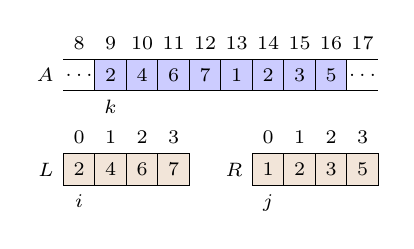
\begin{tikzpicture}
      % array A
      \fill[blue!20!white] (0.8,1.6) rectangle (4.0,2.0);
      \draw (0.4,2.0) -- (4.4,2.0);
      \draw (0.4,1.6) -- (4.4,1.6);
      \foreach \x in {2, 3, 4, 5, 6, 7, 8, 9, 10}
        \draw (\x * 0.4, 1.6) -- (\x * 0.4, 2.0);
      % index texts
      \foreach \x in {8, 9, 10, 11, 12, 13, 14, 15, 16, 17}
        \draw (\x*0.4 - 2.6, 2.0) node[anchor=south] {\scriptsize $\x$};
      \draw (0.4,1.8) node[anchor=east] {\scriptsize $A$};
      \draw (0.6,1.8) node {\scriptsize $\ldots$};
      \draw (4.2,1.8) node {\scriptsize $\ldots$};
      \draw (1.0,1.6) node[anchor=north] {\scriptsize $k$};
      % array contents
      \draw (1.0,1.8) node {\scriptsize $2$};
      \draw (1.4,1.8) node {\scriptsize $4$};
      \draw (1.8,1.8) node {\scriptsize $6$};
      \draw (2.2,1.8) node {\scriptsize $7$};
      \draw (2.6,1.8) node {\scriptsize $1$};
      \draw (3.0,1.8) node {\scriptsize $2$};
      \draw (3.4,1.8) node {\scriptsize $3$};
      \draw (3.8,1.8) node {\scriptsize $5$};

      % array L
      \fill[brown!20!white] (0.4,0.4) rectangle (2.0,0.8);
      \draw (0.4,0.4) -- (0.4,0.8) -- (2.0,0.8) -- (2.0,0.4) -- (0.4,0.4);
      \foreach \x in {2, 3, 4}
        \draw (\x * 0.4, 0.4) -- (\x * 0.4, 0.8);
      % index texts
      \foreach \x in {0, 1, 2, 3}
        \draw (\x*0.4 + 0.6, 0.8) node[anchor=south] {\scriptsize $\x$};
      \draw (0.4,0.6) node[anchor=east] {\scriptsize $L$};
      \draw (0.6,0.4) node[anchor=north] {\scriptsize $i$};
      % array contents
      \draw (0.6,0.6) node {\scriptsize $2$};
      \draw (1.0,0.6) node {\scriptsize $4$};
      \draw (1.4,0.6) node {\scriptsize $6$};
      \draw (1.8,0.6) node {\scriptsize $7$};

      % array R
      \fill[brown!20!white] (2.8,0.4) rectangle (4.4,0.8);
      \draw (2.8,0.4) -- (2.8,0.8) -- (4.4,0.8) -- (4.4,0.4) -- (2.8,0.4);
      \foreach \x in {8, 9, 10}
        \draw (\x * 0.4, 0.4) -- (\x * 0.4, 0.8);
      % index texts
      \foreach \x in {0, 1, 2, 3}
        \draw (\x*0.4 + 3.0, 0.8) node[anchor=south] {\scriptsize $\x$};
      \draw (2.8,0.6) node[anchor=east] {\scriptsize $R$};
      \draw (3.0,0.4) node[anchor=north] {\scriptsize $j$};
      % array contents
      \draw (3.0,0.6) node {\scriptsize $1$};
      \draw (3.4,0.6) node {\scriptsize $2$};
      \draw (3.8,0.6) node {\scriptsize $3$};
      \draw (4.2,0.6) node {\scriptsize $5$};
    \end{tikzpicture}
    \caption{a}
  \end{figure}
\end{frame}

\end{document}
